This exercise focuses on conversion from a color image to a black and white image.
Color images, are often represented by the intensity of red, green and blue also called RGB values.
The value zero represents an absent color and 255 saturated color, so if all RGB values are zero, the the pixel is black, and if all values are 255, then pixel is white.
In the exercise it is recommended to do the conversion with the following formula instead of simply averaging the RGB values.
This is because the human does not perceive colors equally.
\begin{align*}
I = 0.229\cdot R + 0.587\cdot G + 0.114\cdot B
\end{align*} 
In \cuda{} a pixel can be represented by a struct \textit{uchar4} that holds four members, x (red), y (green), z (blue) and w (alpha: component that describes the transparency).
The \textit{w} component is not relevant when converting to gray scale.

\noindent The result of the conversion can be seen in \autoref{fig:ex1} and the source code in \cite{exercises}.
\begin{figure}[ht]
	\centering
	\begin{subfigure}{.5\textwidth}
		\centering
		\fbox{
			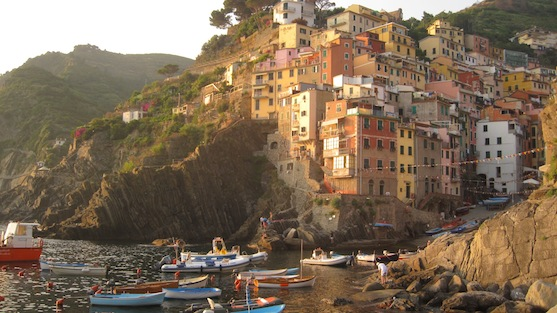
\includegraphics[width=0.7\textwidth]{figs/exercises/ex2/cinque_terre_small.jpg}
		}
		\caption{Before}
		\label{fig:ex1-before}
	\end{subfigure}%
	\begin{subfigure}{.5\textwidth}
		\centering
		\fbox{
			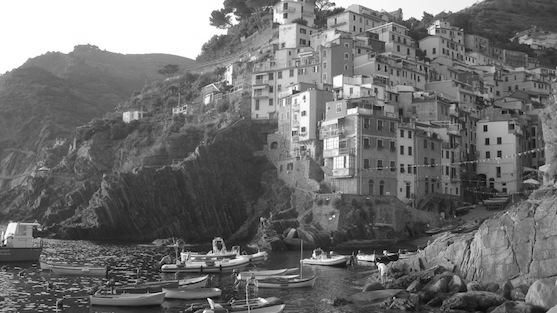
\includegraphics[width=0.7\textwidth]{figs/exercises/ex1/HW1_output.png}
		}
		\caption{After}
		\label{fig:ex1-after}
	\end{subfigure}
	\caption{Picture before and after conversion to gray scale}
	\label{fig:ex1}
\end{figure}
The following steps are performed to solve the exercise.
\begin{enumerate}
	\item[\textbf{Step 0}]
	Write a kernel that converts the pixels from RGB to gray scale.
	This can be done by generating a unique id for each thread, depending on the blockIdx, blockDim and threadIdx in both x and y which determines the pixel to convert.
	When it has been generated, the pixel RGB value is simply converted using the formula above.
	\item[\textbf{Step 1}]
	Launch the kernel with a reasonable block and grid size.
	As the picture is relatively large, it could be beneficial to create the block size as $32\times32$ (1024 is the maximum number of threads in a block) threads and then a grid of blocks depending on the number of rows and columns of the image.
\end{enumerate}